\documentclass[10pt,a4paper]{article}
\usepackage[utf8]{inputenc}
\usepackage{amsmath}
\usepackage{amsfonts}
\usepackage{amssymb}
\usepackage{graphicx}
\usepackage{tikz}
\author{Friedrich Weber\\
\small fweber@posteo.de}
\title{Superinstructions for the SOMns interpreter}

\usetikzlibrary{trees}
\tikzstyle{every node}=[draw=black,thick,anchor=west]

\newcommand{\sinst}[1]{\textsf{#1}}

\begin{document}
	
\maketitle

\section{Heuristic}

The heuristic consist of two stages: The \emph{context collection} stage and the \emph{candidate detection} stage. They are explained separately in the following.

\subsection{Context Collection}

During execution of the program in question, the modified SOMns interpreter dynamically counts the number of activations for each AST node. Here, it also takes the Java type of the activation result into account. Consider, for example, the following code snippet:
\begin{verbatim}
value:: value + 1
\end{verbatim}
which will be parsed into an AST similar to the one shown in Figure~\ref{fig:increment}. Let us assume that the \textsf{value} slot stores a numeric value represented by a Java \textsf{Long} and let us consider a program run in which the \textsf{LocalVariableReadNode} is activated 100 times. During execution, the dynamic analysis records the fact that the \textsf{LocalVariableReadNode} has been activated 100 times, each time producing a \textsf{Long} value. This analysis is implemented in the \textsf{tools.dym.nodes.TypeCountingNode} and \textsf{tools.dym.profiles.TypeCounter} classes.

After execution, the analysis constructs a set of activation contexts from the execution. For each node in the complete AST, it constructs a \emph{trace} which represents the execution context:

A trace is a sequence of strings and integers and has the general form

\begin{align*}
[ C_0, i_0, C_1, ..., i_{k - 1}, C_{k}]
\end{align*}

in which all $C_i$ are Java node class names and all $i_0$ are child slot indices.

\begin{align*}
[ LocalVariableWriteNode, 0, PrimitiveOperation:+, 0, LocalVariableReadNode]
\end{align*}


\section{Superinstructions}

\subsection{Increment Operation}

The superinstruction \sinst{increment} represents the increment of a local \textsf{Long} variable by a fixed integer.
In other words, the following subtree:

\begin{figure}
	\centering
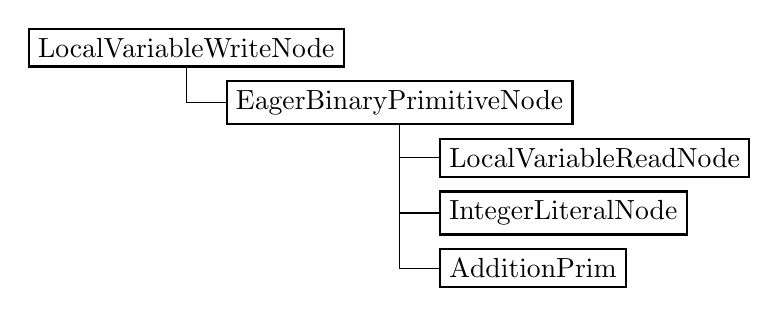
\begin{tikzpicture}[%
grow via three points={one child at (0.5,-0.7) and
	two children at (0.5,-0.7) and (0.5,-1.4)},
edge from parent path={(\tikzparentnode.south) |- (\tikzchildnode.west)}]
\node {LocalVariableWriteNode}
child { node {EagerBinaryPrimitiveNode}
	child { node {LocalVariableReadNode}}
	child { node {IntegerLiteralNode}}
	child { node {AdditionPrim}}
};
\end{tikzpicture}
\caption{AST subtree}
\label{fig:increment}
\end{figure}
	
\end{document}